% !TeX program = pdflatex
% !TeX encoding = UTF-8
% !TeX spellcheck = pt_BR
\documentclass[
  article,
  11pt,
  a4paper,
  english,
  brazil,
  sumario=tradicional]{abntex2}
\usepackage{lmodern}			% Usa a fonte Latin Modern
\usepackage[T1]{fontenc}		% Selecao de codigos de fonte.
\usepackage[utf8]{inputenc}		% Codificacao do documento (conversão automática dos acentos)
\usepackage{indentfirst}		% Indenta o primeiro parágrafo de cada seção.
\usepackage{nomencl} 			% Lista de simbolos
\usepackage{color}				% Controle das cores
\usepackage{graphicx}			% Inclusão de gráficos
\usepackage{microtype} 			% para melhorias de justificação

\usepackage{csquotes}
% ---
% Pacotes de citações
% ---
\usepackage[brazilian,hyperpageref]{backref}	 % Paginas com as citações na bibl
\usepackage[alf]{abntex2cite}	% Citações padrão ABNT
% ---

% ---
% Configurações do pacote backref
% Usado sem a opção hyperpageref de backref
\renewcommand{\backrefpagesname}{Citado na(s) página(s):~}
% Texto padrão antes do número das páginas
\renewcommand{\backref}{}
% Define os textos da citação
\renewcommand*{\backrefalt}[4]{
  \ifcase #1 %
  Nenhuma citação no texto.%
  \or
  Citado na página #2.%
  \else
  Citado #1 vezes nas páginas #2.%
  \fi}%
% ---

% Para fórmulas matemáticas
\usepackage{amsmath}
\usepackage{amssymb}
\usepackage{mathtools}

% Diretório padrão para figuras
\graphicspath{ {images/} }

\hypersetup{
  %hidelinks,   % Comente aqui para exibir os links
  colorlinks, % Descomente esse se comentar o de cima
  linkcolor={red!50!black},
  citecolor={blue!50!black},
  urlcolor={blue!80!black}
}

\usepackage[pdftex,dvipsnames,table,xcdraw]{xcolor}

% Para setas usadas em fórmulas dos grafos
\usepackage{MnSymbol}

% ---
% Altera as margens padrões
% ---
\setlrmarginsandblock{3cm}{3cm}{*}
\setulmarginsandblock{3cm}{3cm}{*}
\checkandfixthelayout
% ---

% --- 
% Espaçamentos entre linhas e parágrafos 
% --- 

% O tamanho do parágrafo é dado por:
\setlength{\parindent}{1.3cm}

% Controle do espaçamento entre um parágrafo e outro:
\setlength{\parskip}{0.2cm}  % tente também \onelineskip

% Espaçamento simples
\SingleSpacing

% Titulo e coisas para cabeçalho
\title{Identificação de Carreiras utilizando Detecção de Comunidades}
\author{Ronie Uliana}

\begin{document}

% Seleciona o idioma do documento (conforme pacotes do babel)
%\selectlanguage{english}
\selectlanguage{brazil}

% Retira espaço extra obsoleto entre as frases.
\frenchspacing

\maketitle

\begin{abstract}
Resumo vai aqui
\end{abstract}

%===================================
\section{Introdução}
%===================================

Carreira profissional e trajetória pessoal

O objetivo desse trabalho é identificar carreiras profissionais a partir de uma rede que representa a movimentação de profissionais entre ocupações.

Essa rede foi gerada pela empresa VAGAS Tecnologia e é explicada em detalhes na Seção~\ref{sec:mapa}. Nela, cada nó representa uma ocupação profissional, as conexões são direcionadas e representam o número de profissionais que passou de uma ocupação para outra em sua trajetória pessoal.



Foram utilizados algoritmos de detecção de comunidades para identificação das carreiras

O modelo ideal de detecção de comunidade permite que um nó faça parte de mais de uma comunidade, desse jeito uma ocupação pode fazer parte de mais de uma carreira. Isso acontece em dois casos: \enquote{Gerente de Projeto} que é uma ocupação homônima para várias carreiras (vide imagem) e \enquote{a-definir} que faz a \enquote{ponte} entre carreiras distintas.

NOTA: Rodei o algoritmo de detecção de comunidade com e sem peso. Os resultados não foram tão bons eu esperava =/. Existem coisas boas ali, mas existe uma certa confusão com os nós mais operacionais. =/

%===================================
\section{Carreira, Fronteira e Permeabilidade} \label{sec:carreira}
%===================================

Segundo~\citeonline{Arthur1989-rn}, carreira é \foreignquote{english}{uma sequência evolutiva da experiência de trabalho de uma pessoa no tempo}\footnote{No original: \enquote{an evolving sequence of person's work experience over time}.}.

Apesar das discussões sobre as mudanças nos modelos de carreira, passando de um modelo linear e centrado na organização para um modelo centrado do indivíduo, as definições de carreira são frequentemente associadas à progressão ou sequência profissional do indivíduo~\cite{Baruch2004-oy,Sullivan2009-xb,Bendassolli2009-bg}.

Para os fins desse trabalho, define-se carreira como \textit{a sequência de ocupações pela qual um indivíduo passa em sua vida profissional}. Essa definição não entra em desacordo com os autores citados, porém, limita a abrangência da definição e a torna mais concreta. Isso permite uma análise menos subjetiva, uma vez que ocupações profissionais podem ser extraídas objetivamente de currículos e analisadas quantitativamente. No entanto, ela se torna mais limitada, já que essa definição exclui aspectos psicológicos ou sociais.

Esse trabalho empresta o conceito de \enquote{barreira} ou \enquote{fronteira} entre ocupações de \citeonline{Gunz2007-hr} e de \enquote{permeabilidade} para dar significado aos resultados do trabalho.

Uma barreira entre ocupações significa que a mudança entre elas não pode ser realizada livremente. Por exemplo, um profissional precisa de graduação especializada antes de poder se mover da ocupação de \enquote{Auxiliar de Jardinagem} para \enquote{Médico}, por outro lado, a barreira para mesmo profissional exercer a ocupação de \enquote{Jardineiro} se restringe à quantidade de experiência. É possível perceber que as barreiras não são simétricas, em um momento de crise é mais simples para uma \enquote{Engenheiro} tornar-se um \enquote{Corretor de Imóveis} do que o contrário.

Barreiras não se limitam ao conhecimento, quaisquer dificuldades na movimentação podem criar fronteiras entre ocupações. Por exemplo, alguém morando em um grande centro urbano dificilmente exerceria a ocupação de \enquote{Agricultor} sem mover-se para o campo. Um \enquote{Diretor Financeiro} precisaria adequar seu padrão de vida antes de se mover para uma ocupação com ganhos mais modestos. Uma profissão que está desaparecendo, como \enquote{Contínuo} possui barreiras mais altas do que uma nascendo, como \enquote{Analista de Experiência do Usuário}.

A permeabilidade entre ocupações está diretamente relacionada à dificuldade em se ultrapassar suas barreiras. Fronteiras permeáveis facilitam a movimentação entre ocupações.

Observando-se a movimentação profissional é possível inferir permeabilidade entre ocupações. Quanto mais profissionais se movem entre elas, mais permeáveis são suas fronteiras. Esse tipo de observação não permite analisar a natureza da barreira, ou seja, o que torna a movimentação fácil ou difícil, mas permite dizer seu grau de permeabilidade.

É esperado, intuitivamente, que carreiras com permeabilidade mais alta entre as ocupações sejam mais frequentes do que carreiras em que ultrapassem barreiras mais altas.

Partindo desse princípio, é possível distinguir conjuntos de ocupações que possuem barreira internas mais baixas entre si do que outras de fora do conjunto. Essa ocupações formam seu próprio domínio, um profissional dentro dele terá mais facilidade de circular entre ocupações do próprio domínio do que sair dele.

%===================================
\section{O Mapa de Carreiras} \label{sec:mapa}
%===================================

O Mapa VAGAS de Carreiras~\cite{VAGAS_Tecnologia2015-yv} é uma rede que resume as movimentações dos profissionais no mercado de trabalho. Nele, cada nó representa uma ocupação e as conexões representam o número de profissionais que se movimentou entre elas, ou seja, nas suas carreiras, deixaram a ocupação anterior e passaram a trabalhar em uma nova.

\begin{figure}[ht]
  \centering
  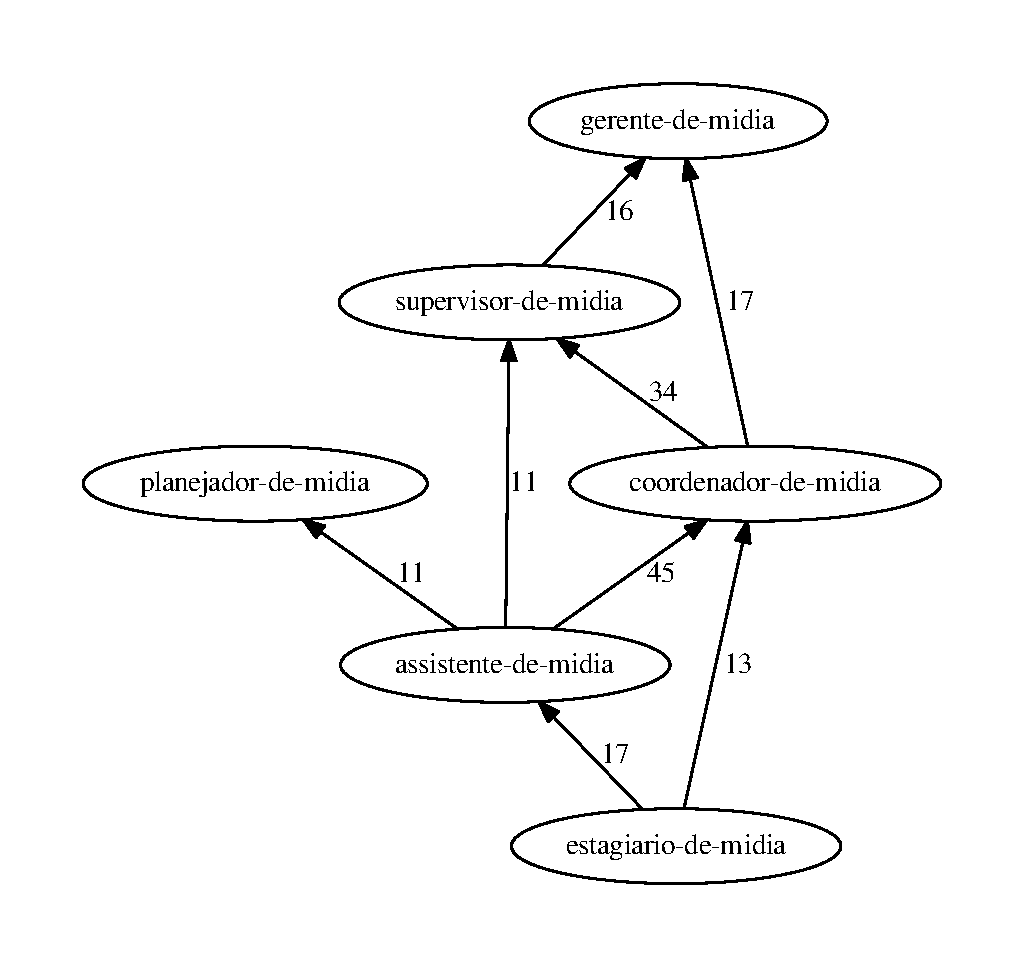
\includegraphics[scale=0.6]{cluster_23.pdf}
  \caption{Parte do Mapa de Carreiras}
  \label{fig:ex-mapa-midia}
\end{figure}

É possível observar parte do Mapa VAGAS de Carreiras (MCar) na Figura~\ref{fig:ex-mapa-midia} com as ocupações relacionadas à profissão de \enquote{mídia}. Nela, por exemplo, 16 pessoas passaram de \enquote{supervisor-de-midia} para a ocupação \enquote{gerente-de-midia}.

O MCar foi gerado a partir dos currículos anonimizados de 10 milhões de usuários registrados no site VAGAS.com.br. A seleção de dados, bem como o processamento das informações, seguiu um procedimento conservador. Isso significa que as decisões tomadas em sua construção procuram minimizar os erros decorrentes da qualidade dos dados.

Da massa de currículos, apenas os atualizados no período entre 2011 e 2016 foram usados. Currículos em duplicação foram removidos usando o CPF como identificador, em caso de duplicação, apenas o currículo mais recente foi considerado. Na impossibilidade de se verificar a duplicação, como por exemplo, na ausência de um identificador, o currículo também foi descartado.

Finalmente, algumas informações gerais foram extraídas dos currículos que sobreviveram ao processo acima e o restante das informações, incluindo possíveis identificadores, foi descartado.

A informações extraídas são o sexo, último salário, graduação (se existente) ou escolaridade, e a sequência de ocupações pelo qual o profissional passou com o título, descrição e período em que exerceu a ocupação.

O título da ocupação é um dos principais artefatos do MCar, é ele quem fornece a identidade para o nó. Nos currículos, o título da ocupação é um campo de texto livre, ou seja, o usuário pode digitar o título sem restrições. Se por um lado isso permite a inserção de ocupações de nicho, novas ou que usem jargão de área; também significa que os títulos possuem erros de grafia, variações de gênero (como em \enquote{advogado} e \enquote{advogada} ou \enquote{moto boy} e \enquote{moto girl}), composição de múltiplas ocupações em um mesmo título (como \enquote{caixa / balconista}), abreviações e toda sorte de erros de interpretação possíveis.

As ocupações passam por um corretor ortográfico criado especificamente para esse trabalho, uma vez que um corretor tradicional não é capaz de identificar jargões de área como \enquote{enfermeiranda}, \enquote{rigger} ou \enquote{IRLA}.

Como exemplo, o dicionário do corretor possui cerca de 750 variações ortográficas que são traduzidas para o termo \enquote{auxiliar}, dentre eles, simples erros de omissão como \enquote{uxiliar} até variações mais elaboradas como \enquote{ausciliar} e \enquote{alsilia}.

Após o trabalho de correção ortográfica, os títulos foram agrupados e contados. Especialistas da empresa verificaram os resultados dos maiores grupos para identificar anomalias como os títulos \enquote{sim}, \enquote{não} e \enquote{o mesmo}, essas ocupações foram excluídas do trabalho.

Finalmente, pares de ocupações foram gerados. Por exemplo, um currículo com a sequência de ocupações \enquote{saladeiro} $\to$ \enquote{chapeiro} $\to$ \enquote{cozinheiro} gera os pares \enquote{saladeiro} $\to$ \enquote{chapeiro} e \enquote{chapeiro} $\to$ \enquote{cozinheiro}.

Os pares foram agrupados para formar o peso de cada conexão na rede final. O peso mínimo 10 foi definido empiricamente para que sejam removidas do mapa as movimentações que incluem erros que o corretor ortográfico não foi capaz de detectar.

Nesse ponto do processo, cerca de 23 milhões de ocupações dos currículos foram agrupadas em pouco mais de 8 mil ocupações distintas.

Finalmente, os pares de ocupações foram conectado entre si a rede final foi construída e armazenada em um banco de dados de grafo. Um sistema online (disponível em http://www.vagas.com.br/mapa-de-carreiras) disponibiliza as informações publicamente.

Apesar de gratuito, os dados do Mapa VAGAS da Carreira não são públicos. A empresa gentilmente cedeu os dados ao pesquisador para esse trabalho.

%===================================
\section{Detecção de Comunidades}
%===================================

Uma comunidade é um subgrafo em que seus nós mais densamente conectados entre si do que a nós que não fazem parte do subgrafo~\cite{Barabasi2016-rn,Ahn2010-uh}.

Uma comunidade é um subgrafo, mas um subgrafo não é necessariamente uma comunidade. A distinção entre um e outro está na conectividade esperada em uma comunidade, o que não é um requisito para subgrafos.

%===================================
\subsection{Comunidades Sobrepostas} \label{sec:comunidades-sobrepostas}
%===================================

Comunidades sobrepostas significa que os nós da rede podem fazer parte de mais de comunidade.

Nesse trabalho, a sobreposição de comunidades possui três papéis específicos: identificação de ocupações \enquote{ponte} entre carreiras, identificação de ocupações homônimas e detecção de sub-comunidades.

Ocupações \enquote{ponte} são aquelas que conectam duas carreiras distintas, a movimentação de uma para outra passa normalmente por essa ocupação.

TK inserir exemplo de ocupação \enquote{ponte}

Por exemplo, na Figura XX é possível observar que a ocupação \enquote{Gerente de Projeto} faz parte de comunidades envolvendo \enquote{design} e \enquote{desenvolvimento de software}.

O papel mais representativo, no entanto está na identificação de sub-comunidades, ou seja, de subgrafos mais fortemente conectados dentro daqueles que já formam uma comunidade. Isso permite a identificação de carreiras mais específicas dentro de grande áreas, como é o caso da comunidade gigante formada por XXXX ocupações.

Para a identificação das características descritas acima, é preciso que os algoritmos permitam a sobreposição e a formação de uma hierarquia entre as comunidades detectadas.

Para medir os melhores pontos de corte nos algoritmos hierárquicos, \citeonline{Barabasi2016-rn} propõem a \textit{Modularidade}, já \citeonline{Ahn2010-uh} propõem a \textit{Densidade de Conexões}.

%===================================
\subsection{Modularidade}
%===================================

A modularidade se baseia nas hipóteses que redes aleatórias não apresentam comunidades distinguíveis e que comunidades são identificáveis unicamente pelo modo como os nós estão conectados entre si, ou seja, duas redes com exatamente o mesmo número de nós e conexões podem apresentar comunidades diferentes. Partindo dessas premissas, a modularidade é calculada como medida de quão os nós dentro da comunidade estão mais densamente conectado entre si do que estariam em uma rede aleatória com características similares.

Para isso, calcula-se a diferença entre a probabilidade de dois nós estarem conectados em uma rede aleatória e a conectividade real entre eles.

A probabilidade $p$ de dois nós $i$ e $j$ estarem conectados em uma rede aleatória (modelo de preservação de grau) depende do grau $k$ de cada nó e do número de conexões $L$ da rede, na forma:

\begin{equation}
p_{ij} = \frac{k_i k_j}{2L}
\end{equation}

A modularidade $M_c$ do subgrafo $C_c$ é definida como:

\begin{equation} \label{eq:modularidade-1}
M_c = \frac{1}{2L} \sum_{(i,j) \in C_c} A_{ij} - p_{ij}
\end{equation}

Onde $A$ é a matriz da adjacência da rede.

Com um pouco de malabarismo matemático (apêndice X), \citeonline{Barabasi2016-rn} derivam a Equação~\ref{eq:modularidade-1} para a forma simplificada:

\begin{equation}
M_c = \frac{L_c}{L} - \left( \frac{K_c}{2L} \right)^2
\end{equation}

Onde $L_c$ é o número de conexões no subgrafo $C_c$ e $K_c$ é a soma de graus dentro do mesmo subgrafo.

A modularidade positiva significa que a o subgrafo $C_c$ possui mais conexões do que o esperado em uma rede aleatória. O valor zero significa que o número de conexões é o mesmo que o esperado em uma rede aleatória e finalmente, um valor negativo significa que uma rede aleatória teria mais conexões que as do subgrafo.

O cálculo da modularidade total da rede é simplesmente a soma da modularidade de todas as comunidades encontradas.

A modularidade possui um limite chamado \enquote{limite de resolução}, \ldots TK completar

%===================================
\subsection{Densidade de Conexões}
%===================================

A densidade de conexões $D_c$ de um subgrafo é o número de suas conexões normalizado pelo valores máximo e mínimo de conexões entre seus nós, ou seja:

\begin{equation}
D_c = \frac{L_c - (N_c - 1)}{L_c (L_c - 1) / 2 - (L_c - 1)}
\end{equation}

Onde $L_c$ e $N_c$ são, respectivamente, o número de conexões e nós do subgrafo.

A densidade máxima de uma comunidade é $1$, significando que ela forma um grafo completo. Um valor $0$ significa que a rede forma uma árvore. Valores negativos indicam que o subgrafo não é uma comunidade, possuindo nós desconectados.

A densidade de conexões total de uma rede é dada pela média ponderada das densidades de todas as comunidades:

\begin{equation} \label{eq:densidade-de-conexoes}
D = \frac{2}{L} \sum_c L_c \frac{L_c - (N_c - 1)}{(N_c - 2) (N_c - 1)}
\end{equation}

Diferentemente da modularidade, a densidade de conexão não possui um limite de resolução.

%===================================
\subsection{Algoritmos para Detecção de Comunidades}
%===================================

Como exposto na Seção~\ref{sec:comunidades-sobrepostas}, o algoritmo selecionado para esse trabalho preserva as características de permitirem hierarquia e o compartilhamento de nós entre diferentes comunidades.

Os algoritmos que permitem hierarquia entre comunidades são baseados em técnicas de agrupamento hierárquico (dendrogramas), \citeonline{Barabasi2016-rn} lista os seguintes algoritmos:

\begin{itemize}
  \item Ravasz - \citeonline{Ravasz2002-qr}
  \item Girvan-Newman - \citeonline{Newman2004-jg}
  \item Link Clustering - \citeonline{Ahn2010-uh}
\end{itemize}

Já os algoritmos que permitem sobreposição de comunidades:

\begin{itemize}
  \item CFinder - \citeonline{Derenyi2005-lb}
  \item Link Clustering - \citeonline{Ahn2010-uh}
\end{itemize}

O algoritmo de agrupamento de conexões (\textit{Link Clustering}) possui as características desejadas para esse trabalho.

\subsection{Algoritmo de Agrupamento de Conexões}

O algoritmo de \citeonline{Ahn2010-uh} agrupa conexões ao invés de nós para a detecção de comunidades. Cada conexão pode participar de um único grupo, porém, como nós podem possuir conexões pertencentes a diferentes grupos eles naturalmente fazem parte de mais da uma comunidade.

Para isso, as conexões são comparadas usando um índice de similaridade e agrupadas utilizando um algoritmo de agrupamento hierárquico. Nesse algoritmo, as conexões de maior similaridade são agrupadas sucessivamente, montando um dendrograma. Ele então é cortado de maneira a maximizar a densidade de conexões $D$ (Equação~\ref{eq:densidade-de-conexoes}), formando as comunidades esperadas.

A similaridade $s$ entre conexões $e_{ik}$ e $e_{kj}$ é calculada pelo índice de Jaccard entre as conexões:

\begin{equation} \label{eq:link-jaccard}
s_{e_{ik} e_{kj}} = \frac{|n_+(i) \cap n_+(j)|}{|n_+(i) \cup n_+(j)|}
\end{equation}

Onde $A$ é a matriz de adjacência, $i$, $k$ e $j$ são nós e a função $n_+(\cdot)$ retorna o próprio nó com seus vizinhos. Na Equação~\ref{eq:link-jaccard} é possível notar que a similaridade é calculada apenas para conexões que compartilham ao menos um nó (representado por $k$). Conexões sem um nó em comum possuem similaridade zero. Na mesma equação, o nó em comum $k$ não aparece explicitamente, mas é levado em consideração por ser um vizinho de $i$ e $j$ e, portanto, fazer parte do retorno da função $n_+(\cdot)$.

A equação de similaridade pode ser generalizada para uma rede ponderada e direcionada. Dado o vetor $\vec{a}_i = (W'_{i1}, \ldots, W'_{iN})$ onde $N$ é o número de nós da rede e

\begin{equation}
W'_{ij} = \begin{dcases}
            \frac{1}{k_i} \sum_{i' \in n(i)} W_{ii'}, & \text{se $i = j$} \\
            W_{ij}, & \text{caso contrário}
          \end{dcases}
\end{equation}

Sendo $W$ a matriz de adjacência com os pesos da rede e $n(i)$ a função que retorna os vizinhos do nó $i$. A similaridade $s^w$ entre duas conexões ponderadas $e_{ik}$ e $e_{kj}$ é:

\begin{equation}
s^w_{e_{ik} e_{kj}} = \frac{\vec{a}_i \cdot \vec{a}_j}
           {|\vec{a}_i|^2 + |\vec{a}_j|^2 - \vec{a}_i \cdot \vec{a}_j}
\end{equation}

\section{Identificação de Carreiras no Mapa de Carreiras}

O trabalho de detecção de comunidades como identificação de carreiras parte das seguintes premissas.

\begin{enumerate}
  \item As ocupações pelas quais um profissional passa em sua carreira compartilham algumas das competências necessárias para exercê-las;
  \item Partindo de uma mesma ocupação, a maior parte dos profissionais seguirá pela próxima ocupação que é mais adequada para suas competências;
  \item Os profissionais têm preferência por ocupações que signifiquem \enquote{progressão}, ou seja, a nova ocupação é profissionalmente superior àquela da qual saiu.
\end{enumerate}

O corolário dessas premissas é que os trajetos mais comuns dos profissionais em suas carreiras identifica o conjunto de ocupações que partilham competências mais fortemente.

Também significa que o sentido de movimentação profissional entre ocupações é o que pode ser considerado \enquote{progressão profissional}.

Essas premissas possuem limitações. Nelas não são consideradas situações de mercado como, por exemplo, ocupações que tendem a desaparecer (como o \enquote{contínuo}) ou aquelas mais afetadas em momentos de crise econômica (como a construção civil).

A partir das premissas e de seus corolários, a detecção de comunidade identifica as ocupações que compartilham competências mais fortemente do que com outras carreiras, o sentido de maior fluxo dentro de uma carreira significa sua direção de progressão.

% Anotações para refinar:

Dois experimentos, com a rede do mapa sem peso ou direção e com a rede apenas sem direção, mas considerando-se o pesos das conexões.

Para e rede simples a similaridade máxima foi de 0,503846 a densidade total $D$ do melhor particionamento possível foi 0,064702. Já para a rede ponderada, a similaridade máxima 0,681787 foi e a densidade 0,024660.

Rede simples:

Similaridade máxima:
Densidade de conexões da rede:
Número de comunidades:
Média de nós nas comunidades:
Quartis de nós nas comunidades:

Rede ponderada:




Ocupações \enquote{ponte} foram encontradas em maior quantidade no início da carreira. É possível observar na Tabela XX o número de ocupações que participam de mais de uma comunidade identificadas como \enquote{estágio}.

TK checar se dá para fazer uma comparação com a nuvem de palavras de cada comunidade.

\section{Conclusões e Perspectivas Futuras}

O fato de ocupações \enquote{ponte} ser encontrada predominantemente no início da carreira pode significar que depois de definido um caminho profissional a movimentação para outra carreira não é feita por movimentações pré-definidas, mas que cada movimentação dessas ocorre de maneira particular. Ao mesmo tempo, indica uma certa mobilidade de escolhas no princípio da carreira.

Os exemplos encontrados de ocupações homônimas indicam uma certa similaridade nas atribuições, mas em especialidades diferentes. TK

\newpage

\bibliography{main}
\end{document}
